\documentclass[11pt,a4paper]{article}
\usepackage[margin=2.35cm]{geometry}
\usepackage[T1]{fontenc}
\usepackage[utf8]{inputenc}
\usepackage{lmodern}
\usepackage{setspace}
\setstretch{1.16}
\setlength{\parskip}{0.35em}
\setlength{\parindent}{1em}
\usepackage{amsmath,amssymb}
\usepackage{booktabs}
\usepackage{tikz}
\usetikzlibrary{arrows.meta,positioning}
\usepackage[hidelinks]{hyperref}

\title{Multi-Factor Model-Predictive Coordination for a Wooden Seed Sowing Machine}
\author{}
\date{}

\begin{document}
\maketitle
\thispagestyle{empty}

\begin{abstract}
\noindent
Vacuum, vibration, and depth are usually tuned one laboratory slice at a time, then left as constants on the machine. Wooden seeds make that practice fail in opposite directions at once: a vacuum that seats a small acorn doubles it in a large cell, and a vibration that unlocks a heavy seed fluidises a light one. This short paper specifies a slow coordinator that chooses shaker frequency and assist vacuum by minimising a logistic cost of miss probability, double probability, spacing scatter, and actuator effort. Depth is held by a servo at 30~mm. The search is blind to any vision constraint on feed speed, so it cannot hide a bad regime behind a slower wheel. On the numerical model of the parent thesis, the coordinator selects zero vacuum in every reported lot. Under a mild 6~Hz disturbance it selects about 9~Hz for red oak and raises planting efficiency from 61\% with speed tracking alone to 77\%. Under a 16~Hz disturbance the 3~Hz and 9~Hz costs nearly tie, and the recorded run selects 3~Hz, lifting efficiency from 22\% to 64\%. The figures are model solutions, not a field trial. They rank a constrained search against a fixed cereal default.
\end{abstract}

\section{Introduction}

A precision meter has more than one input. Shaft speed sets the release rate. Vacuum, vibration, and opener depth change whether a cell fills and whether the seed stays where it was placed. Cereal studies map these factors with response surfaces and publish a setpoint \cite{yazgi2007,karayel2004}. Vibration studies find a frequency above which a rapeseed meter loses discharge, near 10~Hz in one hole-wheel rig, while an irregular vegetable seeder is helped by 50~Hz and a substantial suction \cite{zhang2024,li2025,wu2022}. Copying either setpoint onto an acorn is a category error. A pneumatic hardwood meter metered pin oak and red oak and failed on bur oak and black walnut \cite{wells1990}. The cell did not change in the field.

Model-predictive control was built to re-solve a constrained problem as the measurements move \cite{garcia1989,camacho2007,qin2003}. This paper uses the smallest version that matches the sensors on a single-row wooden-seed planter: one statistical step, an exhaustive grid, and a slew limit. The feed-speed loop is a different paper. Here the shaft is assumed to track the kinematic command. The contribution is the factor decision.

\section{Prediction and cost}

Diameter errors relative to the 24~mm cell are $\delta_{+}=\max(d-d_c,0)/d_c$ and $\delta_{-}=\max(d_c-d,0)/d_c$. A preferred agitation falls as the seed grows,
\begin{equation}
f^{\star}(d)=\mathrm{clip}(4+5\,d_c/d,\ 3,\ 11)\ \text{Hz},
\label{eq:fs}
\end{equation}
and $a=\exp(-((f-f^{\star})/2.6)^2)$ is near one only near that preference. The frequency the seed mass feels combines terrain and the shaker,
\begin{equation}
f_{\mathrm{eff}}=\sqrt{\alpha^2 f_{\mathrm{dist}}^2+f^2}.
\label{eq:fe}
\end{equation}
On the plant, with the coordinator on, $\alpha=0.55$ represents an isolated box mount. The search uses a slightly worse mount, $\alpha^2=0.35$, so it plans pessimistically. Harshness is $H=\max(f_{\mathrm{eff}}-10,0)/10$, using the 10~Hz anchor from the rapeseed rig as a modelling choice, not as a measured acorn resonance \cite{zhang2024}.

Miss and double log-odds are linear in these terms. The miss predictor penalises oversize, harshness, slip, depth error, and a feed scale far from one, and it credits agitation, especially for oversized seeds. The double predictor penalises undersize and vacuum, with vacuum multiplied by $(0.4+\delta_{-})$ so that a few kilopascals hurt a small seed and do little when the seed fills the cell. Probabilities are logistic. The coordinator evaluates them at three diameters, the running mean and the mean shifted by the lot coefficient of variation, with weights $1/2$, $1/4$, and $1/4$. Vision is forced off inside this evaluation, and the feed scale is held at one. The cost is
\begin{equation}
J=\sum_i w_i\big(9p_m^{(i)}+6p_d^{(i)}+4\varsigma^{(i)}/X_t+0.004f+0.01P\big).
\label{eq:J}
\end{equation}
Depth is not searched. A servo holds 30~mm, and the value of that servo in the estimate is a depth noise of 1.2~mm instead of 6.5~mm. The grid is $f\in\{2,3,\ldots,12\}$~Hz and $P\in\{0,1,2,3.5,5\}$~kPa, fifty-five points. The first move is applied and the problem is solved again 200~ms later \cite{mayne2000}. Frequency may change by at most 2~Hz per step, which stops a near-tie from chattering the shaker.

At the nominal red-oak diameter, a 6~Hz terrain, and the pessimistic weight, $J$ is 2.17 at 9~Hz and 0~kPa, against 3.05 at 3~Hz and 0~kPa. Every pressure above zero is worse in that slice. At a 16~Hz terrain the costs at 3~Hz and 9~Hz differ only in the fourth digit. Middle frequencies are worse. The search therefore rejects the middle of the band and rejects a standing vacuum. It does not, on this cost, identify a unique frequency once the frame is already shaking.

\section{What the coordinator is not allowed to see}

The instantaneous bridge index is withheld. If the cost could see it, the search would learn to leave a bridge in place and let a feed constraint clean it up, which looks good in a joint predictor and poor in seeds per minute. The tube count of the last second is also withheld. That count is the outcome. A slow trim of the logistic intercepts, over a minute, would be a reasonable later adaptation. It is not part of this design. Health bits pass between computers. They change mode. They do not enter $J$ as if they were diameters.

A late search keeps the previous feasible $(f,P)$. Holding a feasible input is the standard missed-sample fallback \cite{rawlings2017}. The 55 evaluations are cheap beside a 200~ms period, so a late result is a fault rather than the normal path. The factor task must not run inside the motor interrupt. An overrun there would recreate, on the factor side, the deadline failure already known for combined vision and motion.

\begin{figure}[ht]
\centering
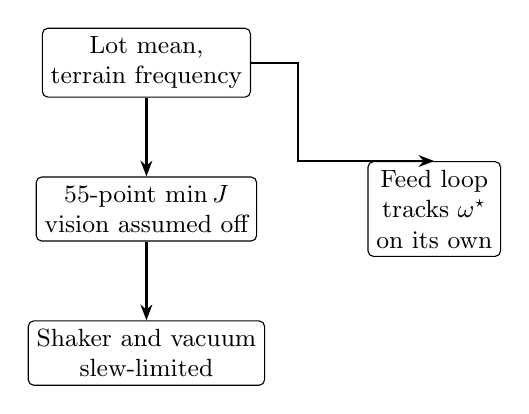
\begin{tikzpicture}[
  font=\small,
  box/.style={draw, rounded corners=2pt, align=center, minimum height=8mm, inner sep=3pt},
  arr/.style={-{Stealth[length=2mm]}, thick}
]
\node[box] (m) {Lot mean,\\terrain frequency};
\node[box, below=10mm of m] (j) {55-point $\min J$\\vision assumed off};
\node[box, below=10mm of j] (a) {Shaker and vacuum\\slew-limited};
\node[box, right=14mm of j] (w) {Feed loop\\tracks $\omega^{\star}$\\on its own};
\draw[arr] (m) -- (j);
\draw[arr] (j) -- (a);
\draw[arr] (m.east) -- ++(6mm,0) |- (w.north);
\end{tikzpicture}
\caption{The factor search does not read the bridge index. The feed loop may still apply one, but the cost is not allowed to count on it.}
\end{figure}

\section{Estimate}

The plant is the same logistic map, integrated for 4{,}000 events with seed 20261029. The coordinator sees the lot mean and coefficient of variation, not the next seed. Slip is rejected by the electronic drive except for a small residual. Table~\ref{tab:m} compares speed tracking at the fixed defaults $f=0$ and $P=3$~kPa with the search.

\begin{table}[ht]
\centering
\caption{Factor coordination against electronic tracking with fixed factors. Efficiency $\eta_{\mathrm{E}}$ is a percentage. The search command is the recorded run.}
\label{tab:m}
\small
\begin{tabular}{@{}lrrrrl@{}}
\toprule
Case & PID $\eta_{\mathrm{E}}$ & MPC $\eta_{\mathrm{E}}$ & MPC $Q_{\mathrm{f}}$ & Miss & Command \\
\midrule
Red oak, 6~Hz & 61.0 & 76.6 & 77.1 & 10.9 & 9~Hz, 0~kPa \\
Red oak, 12$^\circ$ & 60.5 & 75.8 & 77.3 & 11.3 & 9~Hz, 0~kPa \\
Red oak, 16~Hz & 21.8 & 64.5 & 67.2 & 16.6 & 3~Hz, 0~kPa \\
Pin oak, 6~Hz & 61.6 & 75.2 & 70.0 & 10.6 & 10~Hz, 0~kPa \\
Bur oak, harsh & 11.9 & 44.0 & 61.3 & 31.2 & 7~Hz, 0~kPa \\
Mixed, harsh & 37.8 & 65.2 & 68.0 & 16.3 & 8~Hz, 0~kPa \\
\bottomrule
\end{tabular}
\end{table}

Speed tracking recovers a slope, which is why the 12$^\circ$ PID efficiency matches the level row, and it does little about vibration or seed size. The search is the large step. Zero vacuum in every row is the map refusing a cereal default that doubles a small seed in a 24~mm cell. Nine hertz on mild red oak is the preferred agitation of Equation~\eqref{eq:fs}. Three hertz on the 16~Hz row is the quiet side of the near-tie: the sample mean broke the tie toward 3~Hz, and on the plant, with $\alpha=0.55$, that command keeps $f_{\mathrm{eff}}$ near 9.3~Hz while 9~Hz would push it near 12.6~Hz. A second draw can select 9~Hz. The efficiency gain over a silent shaker remains either way. Bur oak still misses about 31 percent of spacings. The cell did not grow. The claim is a recovery from 12\% efficiency to 44\%, not a maize-grade meter \cite{wells1990,kachman1995}.

The energy proxy $0.08\omega^2+0.012f^2+0.02P^2$ is about 0.60 per event for tracking and about 1.40 when the shaker runs at 9~Hz. At the 3~Hz harsh-case command it falls near 0.53, below tracking, because the optimiser has chosen the quiet point. The prices in Equation~\eqref{eq:J} are what make a tie prefer less actuation. They are not a wattmeter.

\section{A printed slice of the cost}

Table~\ref{tab:grid} is the mild red-oak slice at the nominal diameter 20.5~mm, coefficient of variation 0.15, terrain frequency 6~Hz, and the pessimistic terrain weight. It is the same cost the long runs minimise. The corner at 9~Hz and 0~kPa is the minimum of the printed points. Twelve hertz is worse than 3~Hz because $f_{\mathrm{eff}}$ crosses 10~Hz. Raising vacuum never helps this diameter: the double term has a benefit of zero for extra pressure when the vision flag is off, and the price per kilopascal makes a useless vacuum strictly worse. The long-run command for mild red oak matches this corner. The harsh-case near-tie is not in the table, and it should not be smoothed into the same sentence. Mild terrain has a clear frequency. Harsh terrain has two acceptable ends of the range and a bad middle.

\begin{table}[ht]
\centering
\caption{Predicted cost $J$ for nominal red oak at 6~Hz terrain. Lower is better.}
\label{tab:grid}
\small
\begin{tabular}{@{}lrrrr@{}}
\toprule
$f$ (Hz) & $P=0$ & $P=2$ & $P=3.5$ & $P=5$ \\
\midrule
3 & 3.05 & 3.27 & 3.44 & 3.63 \\
6 & 2.84 & 3.05 & 3.21 & 3.39 \\
9 & 2.17 & 2.35 & 2.49 & 2.66 \\
12 & 3.22 & 3.39 & 3.53 & 3.69 \\
\bottomrule
\end{tabular}
\end{table}

\section{Conclusion}

The coordinator is a one-step constrained search over shaker frequency and assist vacuum, with depth removed from the search by a servo. It is predictive control in the receding-horizon sense and a lookup in implementation. Withholding the bridge index is part of the design: the factor regime has to be good when the feed loop is only tracking. The estimate says that regime is low-frequency agitation matched to seed size, no assist vacuum on this cell, and a refusal to add shaker frequency on top of an already harsh frame. A bench that reversed the sign of frequency would refute the shape of Equation~\eqref{eq:fs} and would not, by itself, refute the grid, the slew, or the separation from the feed loop. Those are the parts that remain if the coefficients are replaced by measurements.

\begin{thebibliography}{10}
\bibitem{yazgi2007} A.~Yazgi and A.~Degirmencioglu, ``Optimisation of the seed spacing uniformity performance of a vacuum-type precision seeder using response surface methodology,'' \emph{Biosyst.\ Eng.}, vol.~97, no.~3, pp.~347--356, 2007.
\bibitem{karayel2004} D.~Karayel, Z.~B.~Barut, and A.~\"Ozmerzi, ``Mathematical modelling of vacuum pressure on a precision seeder,'' \emph{Biosyst.\ Eng.}, vol.~87, no.~4, pp.~437--444, 2004.
\bibitem{zhang2024} L.~Zhang, Y.~Liu, M.~Wu, and Z.~Wu, ``Sowing performance of a rapeseed planter under vibration,'' \emph{Appl.\ Sci.}, vol.~14, no.~12, art.~5091, 2024.
\bibitem{li2025} Y.~Li, Y.~Liu, Y.~Ning, H.~Wu, and Y.~Zhao, ``Air-suction drum-type seedling seeder for irregular-shaped vegetable seeds,'' \emph{Sci.\ Rep.}, 2025.
\bibitem{wu2022} W.~Wu et al., ``Seed-filling characteristics of a centralized seed-metering device caused by vibration,'' \emph{Agriculture}, vol.~12, no.~7, art.~965, 2022.
\bibitem{wells1990} L.~G.~Wells, T.~W.~Richards, T.~D.~Smith, and G.~B.~Day, ``Pneumatic metering of hardwood tree seeds,'' \emph{Appl.\ Eng.\ Agric.}, vol.~6, no.~2, pp.~239--243, 1990.
\bibitem{garcia1989} C.~E.~Garc\'ia, D.~M.~Prett, and M.~Morari, ``Model predictive control: Theory and practice---a survey,'' \emph{Automatica}, vol.~25, no.~3, pp.~335--348, 1989.
\bibitem{camacho2007} E.~F.~Camacho and C.~Bordons, \emph{Model Predictive Control}, 2nd ed. Springer, 2007.
\bibitem{qin2003} S.~J.~Qin and T.~A.~Badgwell, ``A survey of industrial model predictive control technology,'' \emph{Control Eng.\ Pract.}, vol.~11, no.~7, pp.~733--764, 2003.
\bibitem{mayne2000} D.~Q.~Mayne, J.~B.~Rawlings, C.~V.~Rao, and P.~O.~M.~Scokaert, ``Constrained model predictive control: Stability and optimality,'' \emph{Automatica}, vol.~36, no.~6, pp.~789--814, 2000.
\bibitem{rawlings2017} J.~B.~Rawlings, D.~Q.~Mayne, and M.~Diehl, \emph{Model Predictive Control: Theory, Computation, and Design}, 2nd ed. Nob Hill, 2017.
\bibitem{kachman1995} S.~D.~Kachman and J.~A.~Smith, ``Alternative measures of accuracy in plant spacing,'' \emph{Trans.\ ASAE}, vol.~38, no.~2, pp.~379--387, 1995.
\end{thebibliography}

\end{document}
